\documentclass[10pt]{article}
\usepackage[utf8]{inputenc}
\usepackage[T1]{fontenc}
\usepackage{lmodern}
\usepackage{listings}
\usepackage{makeidx}
\usepackage[toc, page]{appendix}
\usepackage{float}
\usepackage{lscape}
\usepackage{csquotes}
\usepackage{soul}
\usepackage{textcomp}
\usepackage{gensymb}
\usepackage{pdfpages}
\usepackage{caption}
\usepackage{subcaption}
\usepackage{url}
\lstset{
	keywords={SELECT, WHERE, COLUMNS, ROWS, ON, MEMBER, WITH, FROM, ALL, CROSSJOIN, TOPCOUNT, ASC, DESC, AS, PARENT, CURRENTMEMBER, CHILDREN, PREVMEMBER, NEXTMEMBER, ORDER, RANK, GENERATE},
	keywordstyle=\color{red}\bfseries
}
% \usepackage{geometry}
\usepackage[left=20mm, right=20mm, top=25mm, bottom=25mm]{geometry}
\usepackage{rotating}
\usepackage[section]{placeins}
\usepackage{chngcntr,array}
\usepackage{graphicx}
\usepackage{lscape}
\usepackage{dirtree}
\usepackage[
	breaklinks=true,
	colorlinks=true,
	linkcolor=blue,
	urlcolor=blue,
	citecolor=blue,
	bookmarks=true,
	bookmarksopenlevel=2
]{hyperref}
\usepackage{xcolor}
\usepackage{algorithm}
\usepackage{algpseudocode}
\usepackage{amsmath}
\usepackage{amsfonts}
\usepackage{amssymb}

\title{
	Machine Learning
	\\-\\
	Supervised Learning
}
\author{
	\href{mailto:brandon.alves@gatech.edu}{Brandon Alves}
}
\date{\today}

\begin{document}
	\maketitle
	\tableofcontents
	\listoffigures
	\newpage
	\section{Introduction}
		In this article, I will present the results of various Supervised Learning methods applied on two classification problems. Those methods are:
		\begin{itemize}
			\item Decision Trees with some form of pruning;
			\item Neural Networks;
			\item Boosting;
			\item Support Vector Machines;
			\item K-Nearest Neighbors.
		\end{itemize}
		For each of them, I will discuss the results obtained, the pros and cons of using them, and the parameters that were used. I will also discuss the results when applying the methods on the two different datasets. At the end I will also compare the methods between them and highlight the best one for each dataset.

		I will present many plots on this report to show the evolution of the accuracy depending on some parameters. Those plots will be presented in the following way : the hard line represents the median precision value for a given parameter value while the tint area goes from the minimum to the maximum precision value for the given parameter value.
		% The error bar graph will follow the same convention with the center point representing the median value and the error bar going from minimum to maximum values.

		The experiments on this report were performed on a computer with the following specifications:
		\begin{itemize}
			\item CPU : Intel(R) Core(TM) i7-9750H CPU @ 2.60GHz, 6 cores, 12 threads
			\item RAM : 16GB DDR4
			\item GPU : NVIDIA Quadro P620
		\end{itemize}
	\section{Datasets}
		In this article, I will learn over two datasets:
		\begin{itemize}
			\item \href{https://www.kaggle.com/datasets/elakiricoder/gender-classification-dataset}{Gender Classification};
			\item \href{https://www.kaggle.com/code/sngkadam/credit-card-fraud-detection/data}{Credit Card Fraud Detection}.
		\end{itemize}
		\subsection*{Gender Classification}
			This dataset describes some appearence characteritics. It contains 7 features and one output. The features are: long hair, width of the forehead, height of the forehead, wide nose, long nose, thin lips and the distance between nose and lips. The output feature is gender and takes value 1 for male and 0 for female. That dataset is not the most complicated. I thought it would be a good idea to start with a simple dataset to get a better understanding of the methods. It is also a good idea to start with a dataset that is not too big to avoid long training times.
		\subsection*{Credit-Card Fraud Detection}
			This dataset is a credit card fraud detection dataset. The dataset contains transactions made by credit cards in September 2013 by European cardholders. This dataset presents transactions that occurred in two days, where we have 492 frauds out of 284,807 transactions. The dataset is highly unbalanced, the positive class (frauds) account for 0.172\% of all transactions. It contains only numerical input variables which are the result of a PCA transformation. The only features which have not been transformed with PCA are \textit{Time} and \textit{Amount}. Feature \textit{Time} contains the seconds elapsed between each transaction and the first transaction in the dataset. The feature \textit{Amount} is the transaction amount. Feature \textit{Class} is the response variable and it takes value 1 in case of fraud and 0 otherwise.
		\subsection*{Scaling}
			Some methods require the data to be scaled between 0 and 1. It also permits computation to be faster. Both the training and the testing datasets are scaled between 0 and 1. The scaling is done by dividing each value by the maximum value of the dataset. The scaling is done on the training dataset and then applied on the testing dataset.
	\section{Decision Trees}
		In that section I will present the results obtained when using Decision Trees with pruning. We will here discuss the influence of different parameters :
		\begin{itemize}
			\item The maximum depth of the tree;
			\item The minimum number of samples required to split an internal node;
			\item The size of the training set.
		\end{itemize}

		\begin{figure}[]
			\centering
			\begin{subfigure}[]{0.45\columnwidth}
				\centering
				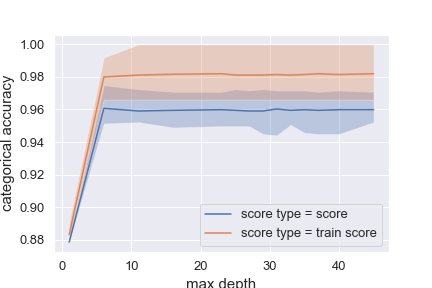
\includegraphics[width=\linewidth]{../graphics/tree_gender_max_depth_score_type_score_type.png}
				\caption{Accuracy for train and test Gender datasets}
				\label{tree:gender_train_vs_test}
			\end{subfigure}
			~
			\begin{subfigure}[]{0.45\columnwidth}
				\centering
				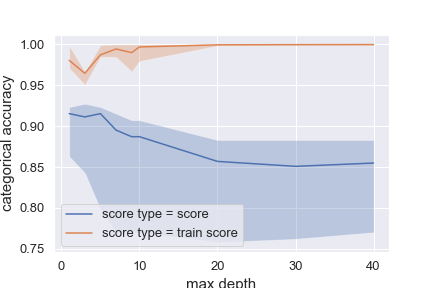
\includegraphics[width=\linewidth]{../graphics/tree_creditcard_max_depth_score_type_score_type.png}
				\caption{Accuracy for train and test Credit-Card datasets}
				\label{tree:creditcard_train_vs_test}
			\end{subfigure}
			\caption{Evolution of the Decision Tree Classifier accuracy according to the Maximum Depth of the Tree}
			\label{tree:train_vs_test}
		\end{figure}

		We begin by finding the limit of our classifier. That limit can be of two natures : overfiting or a flat level on both training and test accuracy. Figure \ref{tree:train_vs_test} represents those limits. On figure \ref{tree:creditcard_train_vs_test}, we can see that the Decision Tree method quickly overfits. Indeed the training accuracy quickly rise above 99\% while the test accuracy decreases to reach around 0.87\%. We can notice that the best score is obtained for a maximum depth value of 5. Also the score considerably decreases for a maximum depth value of bigger than 5. therefore we can conclude that only 5 out of the 28 dimensions of the input space is relevant for the classification output.

		On figure \ref{tree:gender_train_vs_test}, we can notice that the classifier does not overfit. It is interesting to constat the score for the testing dataset happens to be better than the score for the training dataset. This is probably due to the fact that the dataset is not too big. We can also notice that the best score is obtained for a maximum depth value of 7 which means that all the dimensions of the input space are relevant for the classification output.

		\begin{figure}[]
			\centering
			\begin{subfigure}[]{0.45\columnwidth}
				\centering
				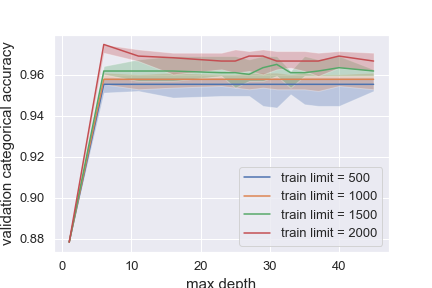
\includegraphics[width=\linewidth]{../graphics/tree_gender_max_depth_score_type_train_limit.png}
				\caption{Accuracy for train and test Gender datasets}
				\label{tree:gender_train_size_score_type_score_type}
			\end{subfigure}
			~
			\begin{subfigure}[]{0.45\columnwidth}
				\centering
				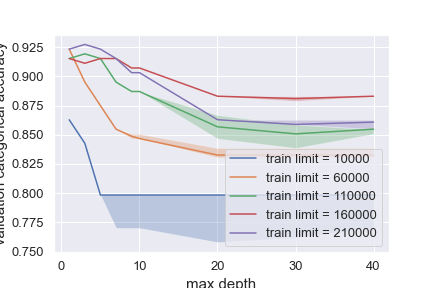
\includegraphics[width=\linewidth]{../graphics/tree_creditcard_max_depth_score_type_train_limit.png}
				\caption{Accuracy for train and test Credit-Card datasets}
				\label{tree:creditcard_train_size_score_type_score_type}
			\end{subfigure}
			\caption{Evolution of the Decision Tree Classifier accuracy according to the Size of the Training Tet}
			\label{tree:train_size_score_type_score_type}
		\end{figure}

		Let's discuss now the influence of the size of the training set on the accuracy of the classifier. Figure \ref{tree:train_size_score_type_score_type} represents the accuracy of the classifier according to the size of the training set for both datasets. As expected the accuracy of the classifier increases when the size of the training set increases. The accuracy of the classifier is also impacted by the maximum depth of the tree. Indeed, the score for all the different sizes of the training set is almost the same when the maximum depth is around 1, whereas the score differs a lot when the maximum depth of the tree increases. We can also notice that the training set with 160 000 samples gives better results than the trainingset with 210 000 samples in figure \ref{tree:creditcard_train_size_score_type_score_type}. This is probably due to the fact that the training set with 160 000 samples is more balanced than the training set with 210 000 samples, meaning that when adding those 50 000 samples, we probably introduce some noise in the training set.

		On the Gender dataset, we can see on figure \ref{tree:gender_train_size_score_type_score_type} that the accuracy of the classifier is also impacted by the size of the training set. The best score of the classifier is for a training set of 2 000 samples. We can also notice that the score is almost the same for a maximum depth between 1 and 5. This means that the training set size as more inpact on the classifier when the maximum depth of the tree is high.

		\begin{figure}[]
			\centering
			\begin{subfigure}[]{0.45\columnwidth}
				\centering
				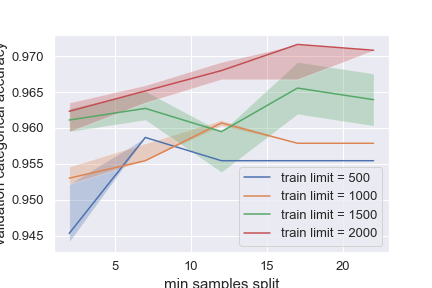
\includegraphics[width=\linewidth]{../graphics/tree_gender_min_samples_split_score_type_train_limit.png}
				\caption{Accuracy for train and test Gender datasets}
				\label{tree:tree_gender_min_samples_split_score_type_train_limit}
			\end{subfigure}
			~
			\begin{subfigure}[]{0.45\columnwidth}
				\centering
				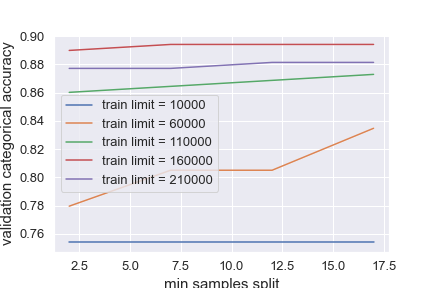
\includegraphics[width=\linewidth]{../graphics/tree_creditcard_min_samples_split_score_type_train_limit.png}
				\caption{Accuracy for train and test Credit-Card datasets}
				\label{tree:tree_creditcard_min_samples_split_score_type_train_limit}
			\end{subfigure}
			\caption{Evolution of the Decision Tree Classifier accuracy according to Minimum Number of Samples required to Split a Node}
			\label{tree:min_samples_split_score_type_score_type}
		\end{figure}

		The last parameter I will discuss is the minimum number of samples required to split an internal node. That variation is displayed on figure \ref{tree:min_samples_split_score_type_score_type}.
		In the Gender dataset, we see that this parameter has some influence. First of all we can see that this parameter lead to overfiting. In the case of the training set composed of 2 000 samples, the classifier overfits for a minimum sample split bigger than 17. But it also improve the results for all the training set sizes, when the minimum sample split is not too high.

		In the case of the Credit-Card dataset, we can see that the accuracy of the classifier is not really impacted by the minimum number of samples required to split an internal node except for the smaller datatset. Which have sense. Indeed, the smaller the dataset is the one with the biggest chance of improvment.

		Decision Tree is the faster method compared with all the other ones. To get those results and generate the data associated with, it took around 10 minutes.

		The decision tree classifier performs pretty well as seen above. But that method does not perform very well on highly dimensional datasets. To resolve that problem, Random Forrest can be used. Random Forrest is a method that uses multiple decision trees to classify the data. The method is based on the idea that a large number of relatively uncorrelated classifiers (trees) operating as a committee will outperform any of the individual classifiers. That method is also known as bagging.
	\section{Neural Networks}
		Neural Network model is the most complicated in terms of parameters in comparison with the other models. We will discuss the influence of the followings:
		\begin{itemize}
			\item The number of epochs;
			\item The use of batch normalization;
			\item The number of layers;
			\item The activation function;
			\item The size of the training set.
		\end{itemize}

		The first thing to say is that our Neural Network classifier does not perform as well as espected with all the parameters explored. For example in the second dataset, in figure \ref{per_sc_train_vs_test}, our classifier difficulty scores above 0.5. As expected the accuracy goes up with the number of epochs.

		\begin{figure}
			\centering
			\begin{subfigure}[]{0.45\columnwidth}
				\centering
				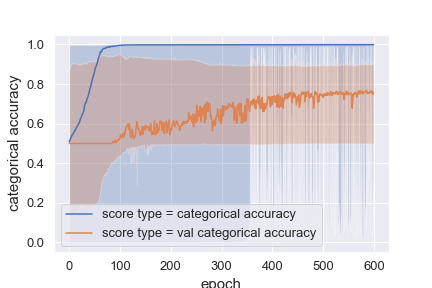
\includegraphics[width=\linewidth]{../graphics/per_creditcard_epoch_score_type_score_type_full.png}
				\caption{Accuracy for the train and test dataset on credit-card}
				\label{per_cc_train_vs_test}
			\end{subfigure}
			\begin{subfigure}[]{0.45\columnwidth}
				\centering
				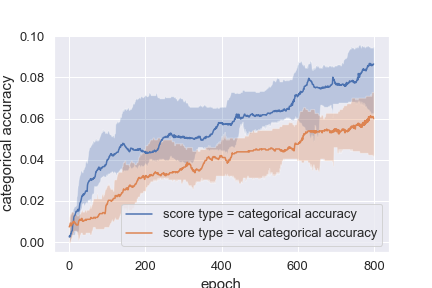
\includegraphics[width=\linewidth]{../graphics/per_starcraft_epoch_score_type_score_type_full.png}
				\caption{Accuracy for the train and test dataset on Starcraft}
				\label{per_sc_train_vs_test}
			\end{subfigure}
			\caption{Evolution of the neural network classifier accuracy according to thenumber of epochs}
			\label{per_train_vs_test}
		\end{figure}

		The parameter that affects the most the accuracy of the calssifier is the use of a batch normalization as we can see on figure \ref{per_cc_bn} and \ref{per_sc_bn}. We know that the use of a batch normalization permits to decrease the number of training epochs required to train a neural network. We can see on figures \ref{per_bn} it decreases drastically the number of epochs.

		\begin{figure}
			\centering
			\begin{subfigure}[]{0.45\columnwidth}
				\centering
				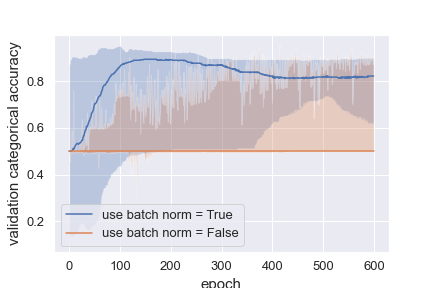
\includegraphics[width=\linewidth]{../graphics/per_creditcard_epoch_score_type_use_batch_norm.png}
				\caption{Accuracy with and without batch normalization for credit-card}
				\label{per_cc_bn}
			\end{subfigure}~
				\begin{subfigure}[]{0.45\columnwidth}
				\centering
				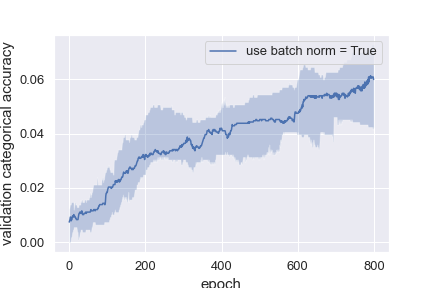
\includegraphics[width=\linewidth]{../graphics/per_starcraft_epoch_score_type_use_batch_norm.png}
				\caption{Accuracy with and without batch normalization for Starcraft}
				\label{per_sc_bn}
			\end{subfigure}
			\begin{subfigure}[]{0.45\columnwidth}
				\centering 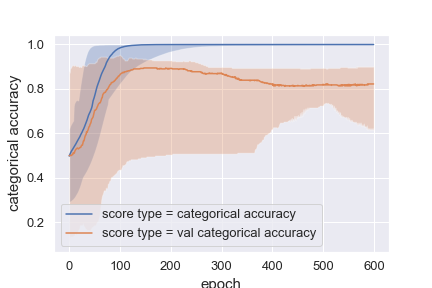
\includegraphics[width=\linewidth]{../graphics/per_creditcard_epoch_score_type_score_type.png}
				\caption{Accuracy for the train and test dataset on credit-card, with batch normalization}
				\label{per_cc_train_vs_test_bn}
			\end{subfigure}~
				\begin{subfigure}[]{0.45\columnwidth}
				\centering
				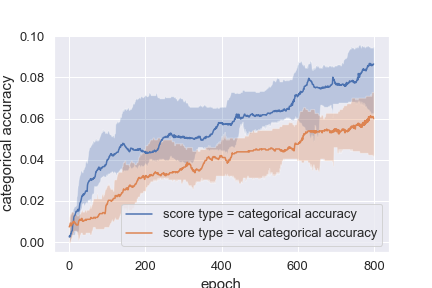
\includegraphics[width=\linewidth]{../graphics/per_starcraft_epoch_score_type_score_type.png}
				\caption{Accuracy for the train and test dataset on Starcraft, with batch normalization}
			\label{per_sc_train_vs_test_bn}
		\end{subfigure}
		\caption{Evolution of the neural network classifier accuracy according to the use of batch normalization}
		\label{per_bn}
		\end{figure}

		The impact of the activation function is not as important as the batch normalization. We can see on figure \ref{per_cc_act} and \ref{per_sc_act} that the accuracy is not very different between the different activation functions expected for the sigmoid function on figure \ref{per_cc_act}.

		Another parameter that affected the score of the classifier was the number of layers. We can see on figures \ref{per_cc_layers} and \ref{per_sc_layers} that for both datasets, the accuracy depends on the layers. One interesting thing to notice is that for Starcraft dataset, the best fit is obtained for no intermediate layers (output neurones directly connected to input) while for credit-card dataset, that configuration gives very poor results.

		One interesting thing in that case is that the training size does not seem to have a big impact on the classification score. We can see on figure \ref{per_cc_tl} and \ref{per_sc_tl} that the accuracy is not very different between the different training sizes. For example we have pretty much the same accuracy for a 1000 and a 160000 training size.

		\begin{figure}
			\centering
			\begin{subfigure}[]{0.45\columnwidth}
				\centering
				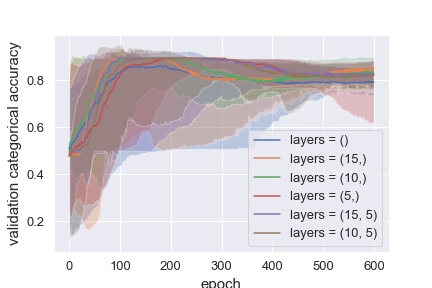
\includegraphics[width=\linewidth]{../graphics/per_creditcard_epoch_score_type_layers.png}
				\caption{Accuracy for different layers on credit-card}
				\label{per_cc_layers}
			\end{subfigure}~
			\begin{subfigure}[]{0.45\columnwidth}
				\centering
				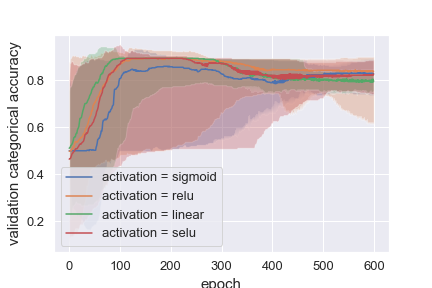
\includegraphics[width=\linewidth]{../graphics/per_creditcard_epoch_score_type_activation.png}
				\caption{Accuracy for different activations on credit-card}
				\label{per_cc_act}
			\end{subfigure}
			\begin{subfigure}[]{0.45\columnwidth}
				\centering
				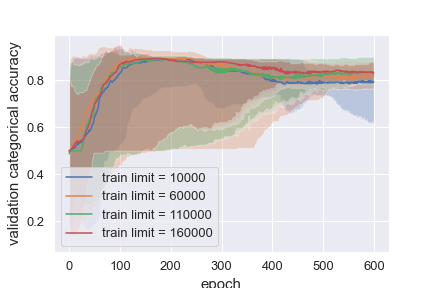
\includegraphics[width=\linewidth]{../graphics/per_creditcard_epoch_score_type_train_limit.png}
				\caption{Accuracy for different training dataset size on credit-card}
				\label{per_cc_tl}
			\end{subfigure}~
			\begin{subfigure}[]{0.45\columnwidth}
				\centering
				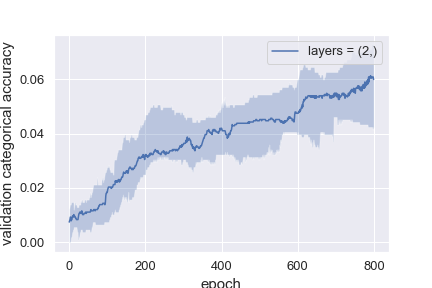
\includegraphics[width=\linewidth]{../graphics/per_starcraft_epoch_score_type_layers.png}
				\caption{Accuracy for different layers on Starcraft}
				\label{per_sc_layers}
			\end{subfigure}
			\begin{subfigure}[]{0.45\columnwidth}
				\centering
				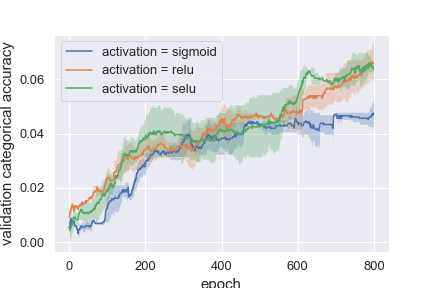
\includegraphics[width=\linewidth]{../graphics/per_starcraft_epoch_score_type_activation.png}
				\caption{Accuracy for different activations on Starcraft}
				\label{per_sc_act}
			\end{subfigure}~
				\begin{subfigure}[]{0.45\columnwidth}
				\centering
				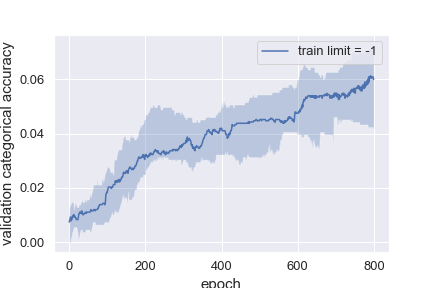
\includegraphics[width=\linewidth]{../graphics/per_starcraft_epoch_score_type_train_limit.png}
				\caption{Accuracy for different training dataset size on Starcraft}
				\label{per_sc_tl}
			\end{subfigure}
			\caption{Evolution of the neural network classifier accuracy for different parameters}
			\label{per}
		\end{figure}

		In terms of computation time, our Neural Network classifier is the slower one. In addition, the memory used in the learning process was also very high. It took 2h30m to train the neural network on both datasets.

		I saw that it was not easy to find a good configuration for the neural network for all these parameters to get good results.
	\section{Boosting}
		Let's now discuss the influence of the followings parameters on the accuracy of the Boosting classifier:
		\begin{itemize}
			\item The number of boosting stages to perform;
			\item The maximum depth of an individual regression estimator;
			\item The minimum number of sample needed to split a node of an estimator;
			\item The size of the training set.
		\end{itemize}
	\section{Support Vector Machines}
		In this section we will discuss about the Support Vector Machines classifier. We will see the influence of the followings parameters:
		\begin{itemize}
			\item The penalty of the error term (C value);
			\item The kernel function;
			\item The training set size.
		\end{itemize}

		\begin{figure}
			\centering
			\begin{subfigure}[]{0.45\columnwidth}
				\centering
				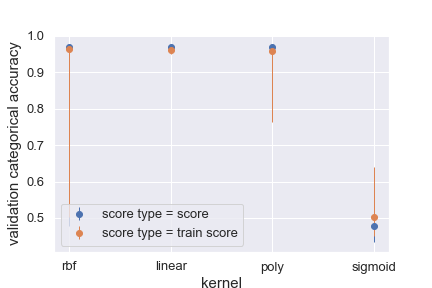
\includegraphics[width=\linewidth]{../graphics/svm_gender_kernel_score_type_score_type.png}
				\caption{Accuracy for the train and test Gender datasets}
				\label{svm:g_train_vs_test}
			\end{subfigure}
			~
			\begin{subfigure}[]{0.45\columnwidth}
				\centering
				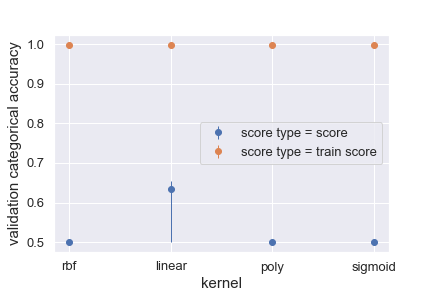
\includegraphics[width=\linewidth]{../graphics/svm_creditcard_kernel_score_type_score_type.png}
				\caption{Accuracy for the train and test Credit-Card datasets}
				\label{svm:cc_train_vs_test}
			\end{subfigure}
			\caption{Evolution of the SVM Classifier accuracy according to the Kernel}
			\label{svm:train_vs_test}
		\end{figure}

		The parameter that seems to have the biggest impact is the kernel choosed.
		In figure \ref{svm:train_vs_test}, we can see the impact on the score for both datasets. In the case of the Gender dataset, on figure \ref{svm:g_train_vs_test}, we see that the accuracy is pretty much the same for all the kernels except for the \textit{sigmoid} where the accuracy falls down to 0.45. The accuracy is around 0.98 for the other kernels : linear, polynomial (3rd degree) and the radial basis function. The score for the linear kernel clearly show that the data are linearly separable.
		In the case of the Credit-Card dataset, on figure \ref{svm:cc_train_vs_test}, we see that the accuracy is better for the linear kernel, with an accuracy around 0.61. The other kernels don't perform very well.

		\begin{figure}
			\centering
			\begin{subfigure}[]{0.45\columnwidth}
				\centering
				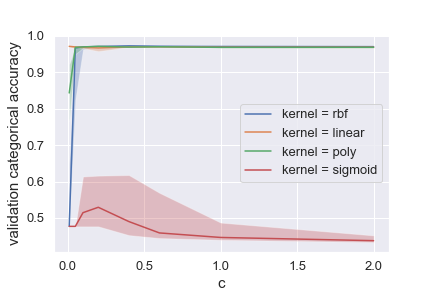
\includegraphics[width=\linewidth]{../graphics/svm_gender_c_score_type_kernel.png}
				\caption{Accuracy for test Gender dataset according to different kernels}
				\label{svm:g_c}
			\end{subfigure}
			~
			\begin{subfigure}[]{0.45\columnwidth}
				\centering
				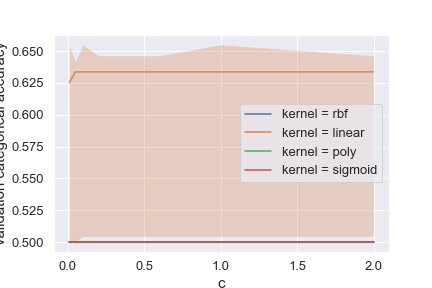
\includegraphics[width=\linewidth]{../graphics/svm_creditcard_c_score_type_kernel.png}
				\caption{Accuracy for test Credit-Card dataset according to different kernels}
				\label{svm:cc_c}
			\end{subfigure}
			\caption{Evolution of the SVM Classifier accuracy according to the C value}
			\label{svm:c}
		\end{figure}

		Let's now study the impact of the C parameter. In SVM, we are searching for a hyperplane with the largest minimum margin, and a hyperplane that correctly separates as many instances as possible. The problem is that it is not always possible to get both. The C parameter determines how great our desire is for the latter. Figure \ref{svm:c} presents the accuracy for the test dataset according to the C value.
		For Gender dataset, we can see, on figure \ref{svm:g_c} that the C value doesn't have a big impact on the accuracy. The accuracy is around 0.98 for all the C values bigger than 0.01, except for the \textit{sigmoid} kernel where the accuracy falls down tunder 0.5. Once again, because the data are linearly separable, the accuracy is pretty much the same for all the C values bigger than 0.01.
		The strength of the regularization is inversely proportional to C. So, the smaller C is, the stronger the regularization is. Having a C value to small means that we are considering the margin too much, and we are not allowing enough errors. So, we are underfitting the data.
		In the case of the Credit-Card dataset, on figure \ref{svm:cc_c}, we can see that the accuracy is neither really affected by the regularisation parameter for both kernels.

		\begin{figure}
			\centering
			\begin{subfigure}[]{0.45\columnwidth}
				\centering
				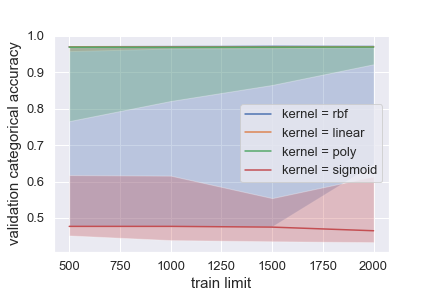
\includegraphics[width=\linewidth]{../graphics/svm_gender_train_limit_score_type_kernel.png}
				\caption{Accuracy for test Gender dataset for different kernels}
				\label{svm:g_train_limit}
			\end{subfigure}
			~
			\begin{subfigure}[]{0.45\columnwidth}
				\centering
				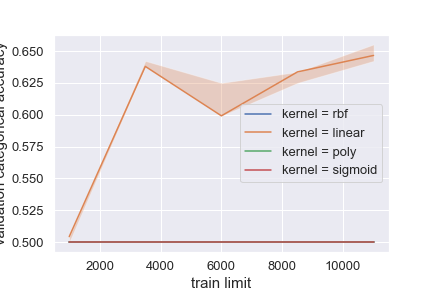
\includegraphics[width=\linewidth]{../graphics/svm_creditcard_train_limit_score_type_kernel.png}
				\caption{Accuracy for test Credit-Card dataset for different kernels}
				\label{svm:cc_train_limit}
			\end{subfigure}
			\caption{Evolution of the SVM Classifier accuracy according to the Size of the Training Set}
			\label{svm:train_limit}
		\end{figure}

		The last parameter I will discuss for SVM is the training size. The results are presented on figure \ref{svm:train_limit}.
		For the Gender dataset, we can see on figure \ref{svm:g_train_limit} that the accuracy is pretty much the same for all the training set sizes, with the working kernels. That dataset is indeed too easely separable.
		For the Credit-Card dataset, we can see on figure \ref{svm:cc_train_limit} that the accuracy for the linear kernel is impacted by the training set size. There is that hollow betwenn 4 000 and 8 000 samples which means that we probably introduced outliers in the data. But the accuracy seems overall increasing with the training set size. I was not able to train more data due to the time computation of the SVM classifier.

		Concerning time efficiency, the SVM classifier achieve a correct performance. To get those results and generate the data associated with, it took around 25 minutes.

		In conlusion, SVM does not perform very well on the most difficult dataset, the Credit-Card one. I think the most important for SVM working well is the choice of the kernel function as seen above. In the overhand, data are not always linearly separable. In the case of the Credit-Card dataset, it seems that it is not the case. So SVM does not seem to be a good option.
	\section{K-Nearest Neighbors}
		Here I will discuss the results obtained using a K-Nearest Neighbors classifier. We will see the influence on the accuracy of the classifier of:
		\begin{itemize}
			\item The number of neighbors;
			\item The distance metric (p-norm);
			\item The size of the training set.
		\end{itemize}
		By design, the accuracy on the training set is always 100\% for KNN, so I will not display it on the plots.

		\begin{figure}
			\centering
			\begin{subfigure}[]{0.45\columnwidth}
				\centering
				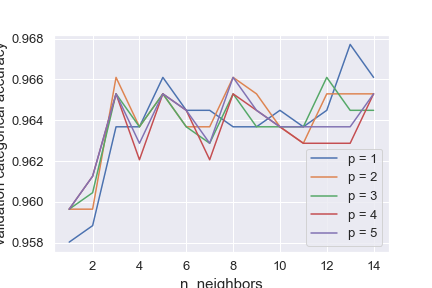
\includegraphics[width=\linewidth]{../graphics/knn_gender_neighbors.png}
				\caption{Evolution of the accuracy according to the number of neighbors on Gender dataset, with $train\_limit = 2000$}
				\label{knn:g_neighbors}
			\end{subfigure}
			~
			\begin{subfigure}[]{0.45\columnwidth}
				\centering
				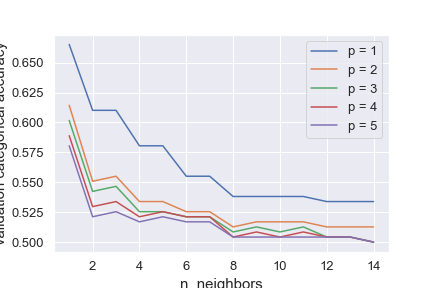
\includegraphics[width=\linewidth]{../graphics/knn_creditcard_neighbors.png}
				\caption{Evolution of accuracy according to the number of neighbors on Credit-Card dataset, with $train\_limit = 90000$}
				\label{knn:cc_neighbors}
			\end{subfigure}
			\begin{subfigure}[]{0.45\columnwidth}
				\centering
				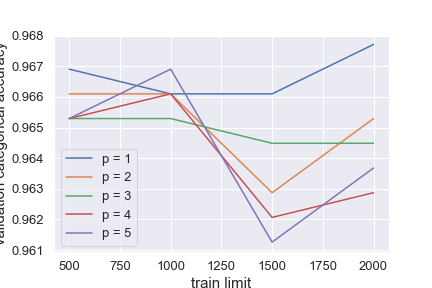
\includegraphics[width=\linewidth]{../graphics/knn_gender_train_limit.png}
				\caption{Evolution of accuracy according to the number of training examples on Gender dataset, with $n\_neighbors = 13$}
				\label{knn:g_train_limit}
			\end{subfigure}
			~
			\begin{subfigure}[]{0.45\columnwidth}
				\centering
				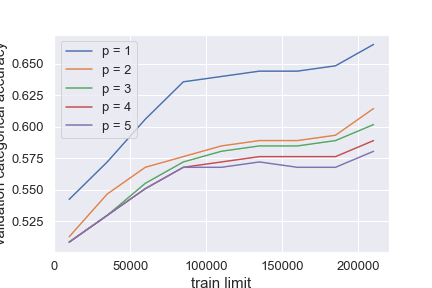
\includegraphics[width=\linewidth]{../graphics/knn_creditcard_train_limit.png}
				\caption{Evolution of accuracy according to the number of training examples on Credit-Card dataset, with $n\_neighbors = 1$}
				\label{knn:cc_train_limit}
			\end{subfigure}
			\caption{Evolution of the K-NN Classifier accuracy on the Test Set for different Parameters}
			\label{knn:knn}
		\end{figure}

		On figure \ref{knn:knn}, I present the effect of those parameters on the classification score.
		For the Credit-Card dataset, we can notice that the norm used for the distance metric has a consequent influence on the classification accuracy. The accuracy is better when using the Manhattan norm ($p = 1$). This is not a surprise as higher norm are generally inadequate to measure distances on highly dimensional spaces. In the case of the Gender datatset, the norm used doesn't seem to have a big influence on the accuracy.

		On figures \ref{knn:cc_neighbors} we can see that the accuracy of the classifier is better for a small number of neighbors. K-NN is a non-parametric classifier. It is not able to generalize the data, so it is better to use a small number of neighbors. We usually increase the research perimeter to be more resilient to noise but here the data do not allow us such a liberty. This is particularly true in the Credit-Card dataset where the fraud are really close to legal transactions. On figure \ref{knn:g_neighbors}, we can see that the accuracy is better for a number of neighbors bigger than 3. In the case of the Gender dataset, the data are more separated and we can afford to increase the number of neighbors.

		On figures \ref{knn:cc_train_limit}, we can see that the accuracy of the classifier is better for an important number of training examples. Also the classifier doesn't overfit. On figure \ref{knn:g_train_limit}, we can see that the accuracy decreases for a number of training examples between 1 000 and 1 500. But it keeps having a very good score. I don't really know why. Maybe the samples introduced where not well representative of the data.

		Concerning time efficiency, the K-NN classifier achieve a correct performance. To get those results and generate the data associated with, it took around 25 minutes.

		In comparison with the other methods, K-NN didn't  perform well on the Credit-Card dataset. Having a discussion with an expert of the dataset would be a good idea for designing a distance metric that is better suited to the problem. Indeed, the distance metric is the key to success with K-NN. So it is important to choose the most appropriate one.
	\section{Conclusion}
\end{document}
